\chapter{Research} \label{questions}
In this chapter, the research questions for the thesis are formulated. What research method will be used, and how the questions are being validated.

\section{Context}
The graduation assignment evolves around change detection and visualising the comparison between version of the application under test. The result is an external application that connects to OrientDB and calculates and shows the model comparison. Figure \ref{fig:components-overview} shows the different components involved. The \textit{New Analysis Website} component is the component that is created. Section \ref{sec:components-explained} explained the different components in more detail.

The external application is built as a separate application next to the \testar application. The code that was created by Pastor Ricós (Section \ref{sec:state-model-difference}) and Mulders (Section \ref{inferred-model}) are used as a starting point for the external application. 

\begingroup
\captionsetup{type=figure}
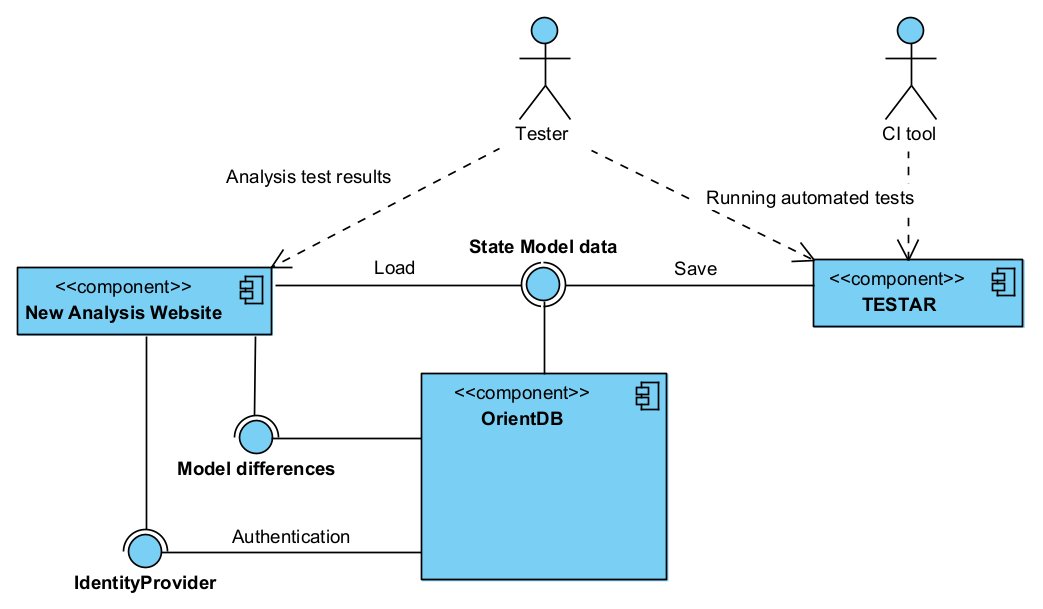
\includegraphics[scale=0.4]{images/3-UML-high-level.png}
\captionof{figure}{Components overview (UML 2.0)}\label{fig:components-overview}
\endgroup

Because change detection is the subject for this graduation assignment, it is assumed that the inferred model generator will generate useful models for change detection. Although the inferred model generator is out-of-scope, it is not ruled out that changes are necessary.

Any automatic learning capabilities are also out-of-scope. A change detection learning capability could be a topic for a future research proposal. Regarding this research proposal, a human will be needed to evaluate the results and outcome of the change detection application.

\section{Research questions} \label{research-questions}
        
The main research question is: \textbf{How can an automated comparison of inferred models help testers finding bugs?}

The main research question is divided into three parts. The first part (\ref{rq:detect-changes}) will research how to detect changes between different versions of the same GUI software (SUT) \cite{testar-todo}. The second part (\ref{rq:diff-visualisation}) will research how to visualise the detected changes. A third Research Question \ref{rq:validation} is dedicated to validating the previous research questions. The research questions are as follows: 


\begin{questions}

    \item How can we set up the change detection as an application written outside of \testar? \label{rq:application-outside-testar}

    \item How to detect changes between two versions of the SUT? \label{rq:detect-changes}
    \begin{questions}
        \item What is change detection, and what do we want to use it for? \label{rq:what-is-change-detection}
        \item Which properties make a model useful for change detection? \label{rq:useful-detection}
        \item Which \testar configuration will generate the useful model? \label{rq:testar-config}
        \item How can we find changes between two models? \label{rq:finding-changes}
    \end{questions}


    
    \item How to visualise the detected differences to the user? \label{rq:diff-visualisation}
    \begin{questions}
        \item What tooling is available to show the result of the change detection? \label{rq:tooling}
        \item How to visualise each change? \label{rq:type-visualisation}
        \item How to generate the shortest set of actions that helps the user to reach the changed state in the SUT? \label{rq:shortest-set}    
    \end{questions}
    
    \item How to validate the results of \ref{rq:detect-changes} and \ref{rq:diff-visualisation}? \label{rq:validation}
    \begin{questions}
        \item What are the requirements for validation applications? \label{rq:req-apps}
        \item Which applications can be used for validation? \label{rq:validation-apps}
    \end{questions}
\end{questions}

\subsection{\ref{rq:application-outside-testar}How can we set up the change detection as an application written outside of \testar?}
\todo{write this section}
extra things had to be done
Industial standards
F-Secure


\subsection{\ref{rq:what-is-change-detection} What is change-detection, and what do we want to use it for?}
To get an answer for \ref{rq:what-is-change-detection}, a literature study will be conducted. The literature study aims to bring an overview of change detection in general and its application in the \testar context. Not only change detection in the GUI but also other change detection methods in the field of Software Engineering, like cross-browser testing. 

\subsection{\ref{rq:useful-detection} Which properties make a model useful for change detection?}
The outcome of \ref{rq:useful-detection} is a list of requirements for the inferred model that are needed to enable change detection. For example, can a non-deterministic state model be used? However, it also includes requirements for the algorithm, like, what are acceptable calculation speeds and how big can a state model be while still complying with the speed requirement? When the set of properties are known, Vaandrager's criteria are used to validate the model \cite{vaandrager}.

\subsection{\ref{rq:testar-config} Which \testar configuration will generate a useful model?}
There are a couple of ways to change the outcome of an inferred model, for example, picking widget attributes for the hash calculation. These configurations can influence the usefulness of the model. The outcome of \ref{rq:useful-detection} should result in a \testar configuration file that configures \testar to generate this useful model. It might be necessary to make code changes in the state model generation or to the identification calculation to implement a Merkle tree approach. Using a Merkle tree could help with comparison to graphs, especially changed in the widget tree. 

A threat of validity for \ref{rq:testar-config} is that every application under test needs its unique configuration. Therefore, it might be wise to look into all widget attributes during the change detection and not take the hash of a state for the comparison. The configuration can be used for tuning the model and the change detection by taking the above approach.

\subsection{\ref{rq:finding-changes} How can we find changes between two models?}
\ref{rq:finding-changes} is the closing question in which the change detection algorithm is coded in Java. In a recent master thesis by Slomp \cite{thesisSlomp}, it is possible to run \testar in a Docker container. As a consequence, \testar can run without a GUI. Therefore the change detection algorithm will run in a separate application, outside the \testar context. The result of the change detection needs to be saved to a data store, preferably the already existing OrientDb database. 

\subsection{\ref{rq:tooling} What tooling is available to show the detected differences?}
Aside from the inferred model, Mulders also created an application to visualise the models. It is essential to state that Mulders did extensive research on which technology fits his needs best. \ref{rq:tooling} will look at the results of Mulders and revalidate whether the libraries are suitable for visualising the differences. 

\subsection{\ref{rq:type-visualisation} How to visualise change?}
\ref{rq:type-visualisation} will look into the execution of the visualisation tool. How can added, removed or altered states in the inferred model be visualised the best? Like \ref{rq:finding-changes} this also includes moving the visualisation tool into its separate application, outside the \testar context. The requirements and GUI proposals will be discussed with the \testar stakeholders. 

\subsection{\ref{rq:shortest-set} How to generate the shortest set of actions that helps the user to reach the changed state in the SUT?}
One of the requirements of the visualisation is showing how to reach the state that has changed. Dijkstra's algorithm \cite{dijkstra1959note} is a well-known algorithm to find the shortest path for a given graph. However, as Goldberg and Harrelson \cite{goldberg2005computing} showed, it is not the most optimal shortest path algorithm, especially with massive graphs. 

\subsection{\ref{rq:req-apps} What are the requirements for validation applications?}
To validate the outcome of the change detection algorithm, we will need to have an application to test it on. The research question will create a set of requirements for the validation application, like multiple versions. The set will be discussed with the supervisors to make sure nothing will be forgotten.

\subsection{\ref{rq:validation-apps} Which applications can be used for validation?}
During development and system testing, the two-button app will be extended and used. Although the app is excellent during the development phase, it is nowhere close to a real-world application. Based on the outcome of \ref{rq:req-apps}, an application needs to be found in order to test the change detection algorithm.

In addition to the application found, F-secure will be asked for feedback on the algorithm and the visualisation. F-Secure is a company based in Finland that provides security solutions to its customers and are currently testing the proof of concept of Pastor Ricós \cite{f-secure}.

With the combination of real-world application and the feedback from F-Secure, biased towards a single point of view for the algorithm will be minimized. 